\documentclass[a4paper,10pt]{article}

\usepackage{titlesec}
\titleformat*{\section}{\large\bfseries}
%\titleformat*{\section}{\LARGE\bfseries}
\titleformat*{\subsection}{\large\bfseries}
%\titleformat*{\subsection}{\Large\bfseries}
\titleformat*{\subsubsection}{\large\bfseries}
\titleformat*{\paragraph}{\large\bfseries}
\titleformat*{\subparagraph}{\large\bfseries}

\usepackage[T1]{fontenc}
\usepackage[utf8]{inputenc}
\usepackage{lmodern}
\usepackage[english]{babel}
%maths :
\usepackage{amssymb,amsmath,amsthm,bm}

\usepackage{pdfpages}

%Réduction des marges
\usepackage[margin=0.5in]{geometry}

%Supression des numéros de page
\pagenumbering{gobble}

\title{Lab 0}
\author{Johannes Lemonde et Lucas Streit}

\begin{document}

\maketitle
%\tableofcontents

%\begin{abstract}
%\end{abstract}

\setcounter{section}{2}
\section{Questions to chapter 3}
\setcounter{subsection}{1}
\subsubsection{Flow diagram for the \texttt{delay} subroutine}

See at the end.

\subsubsection{Calculating \texttt{delaycount} in order to achieve \texttt{1 ms} in \texttt{delay}'s inner-loop}

We have \( \frac{50~[MHz~op]}{4~[\frac{op}{loop}]~1000~[\frac{ms}{s}]} = 12'500 [\frac{loops}{ms}] \), so we would set \texttt{delaycount} to 12'500.

Experimentally, we figured out that it should be set to 860 approx (why?)



\setcounter{subsection}{2}
\setcounter{subsubsection}{0}



\subsubsection{What is BSP and what does it contain?}

BSP means Board Support Package. It is the layer of software containing hardware-specific drivers and other routines that allow a particular operating system to function. It initialises the processor, bus, interrupts, clock, RAM, amongst others, and runs the boot loader.

The BSP project in Eclipse contains amongst others all the files necessary to access the LEDs, switches, buttons, etc.

\subsubsection{What is a soft-core processor? What type of processor is present? Features?}

We talk about soft-core processors when we configure a reprogrammable logic, such as a FPGA, to function as a processor. \\
For these laboratories, we use the NIOS II soft processor, which is a soft microprocessor core for Intel FPGAs.\\
Clock frequency: 50 MHz; neither data nor instruction caches for NIOS  II/e; No pipeline nor branch prediction for NIOS II/e.

\subsubsection{How does the processor access peripherals? What is the main mechanism and what main piece of hardware stands between the processor and a peripheral?} 

Peripherals are accessed through the Avalon Switch Fabric, which lets several masters from the core to operate at the same time. In other words, in handles the requests from the masters to the slaves (peripherals).

\subsubsection{What peripherals/IP cores are present in the provided architecture? Identify their symbolic names and base addresses.}

Buttons, switches, green and red LEDs, seven segment displays, ...
For the symbolic names and base addresses, see \texttt{system.h} (within the BSP project in Eclipse).

\subsubsection{What types of memory are present in the provided architecture? Identify their symbolic names, base addresses and sizes. What are the typical access time for each of these memories?}

On chip memory : \texttt{ONCHIP\_MEMORY\_BASE}, address: \texttt{0x0}, size: \texttt{25600 words}, typical access time: \texttt{1 cycle at 50MHz}.\\
%PERFORMANCE\_COUNTER\_BASE 0x9000 128\\
\\
SDRAM: \texttt{SDRAM\_BASE}, base-address: \texttt{0x1000000}, size: \texttt{8388608 words}, typical access time (CAS latency): \texttt{3 cycles at 50 MHz}.




\setcounter{subsection}{3}
\setcounter{subsubsection}{0}


\subsubsection{What macro is used to write to a parallel I/O port? How about to read from one?}

We can use the macros \texttt{IOWR\_ALTERA\_AVALON\_PIO\_DATA(base, data)} and  \texttt{IORD\_ALTERA\_AVALON\_PIO\_DATA(base)}, defined in \texttt{\$BSP\_PROJECT/drivers/inc/altera\_avalon\_pio\_regs.h}, where \texttt{base} is the address of the port and \texttt{data} is the data to write.

\subsubsection{What command will you use to turn on all red LEDs?}

We have to run the previous command with \texttt{DE2\_PIO\_REDLED18\_BASE} as the \texttt{base} and $(2^{18}-1)$ as the \texttt{data}.
It would look like that: \texttt{IOWR\_ALTERA\_AVALON\_PIO\_DATA(DE2\_PIO\_REDLED18\_BASE, 0x3FFFF);}

\subsubsection{What command would you use to read the current status of all push-buttons?}

\texttt{IORD\_ALTERA\_AVALON\_PIO\_DATA(D2\_PIO\_KEYS4\_BASE);}, where the function returns a 4 bit number, each bit corresponding to the status of one push-button, \texttt{0} meaning currently pushed and \texttt{1} meaning released. 

\subsubsection{Which header file do you need to include in your program to access the symbolic names? What about the read/write macros?}

Basically, \texttt{"system.h"} defines the base-addresses of the peripherals (symbolic names), such as for instance \texttt{D2\_PIO\_KEYS4\_BASE}, and \texttt{"altera\_avalon\_pio\_regs.h"} defines the macros to read/write.

\setcounter{subsection}{6}
\setcounter{subsubsection}{0}
\subsubsection{What is the IRQ level for buttons?}

\texttt{\#define D2\_PIO\_KEYS4\_IRQ 8} in the \texttt{system.h} file.

\subsubsection{Which other peripherals support interrupts?}

The toggles (IRQ 6), the JTAG UART (IRQ 5), Timer 0 (IRQ 7), Timer 1 (IRQ 9).
(found in \texttt{system.h}).


\setcounter{section}{5}
\setcounter{subsection}{1}
\setcounter{subsubsection}{0}

\subsubsection{How are the timestamp timer and the performance counter functioning? Describe the main steps.}

The timestamp is basically a counter which gets incremented -- in this case -- at every tick of the clock.

The performance counter is a peripheral containing several counters allowing to count the number of ticks within a section of code chosen for analysis, without 



Results :

\begin{tabular}{c||c|c}
    & Time (ms) & Error (ms) \\
    \hline
    \hline
    Timestamp timer & 54.222 & 0.273 \\
    \hline
    Performance counter & 54.202 & 0.258
\end{tabular}



\begin{tabular}{c||c|c}
    Flag & Time (ms) & Size (KB) (ELF file) \\
    \hline
    \hline
    -O0 & 50.195 & 80.876 \\
    \hline
    -O2 & 10.898 & 80.356\\
    \hline
    -Os & 10.950 & 80.308
\end{tabular}

\setcounter{subsection}{3}
\setcounter{subsubsection}{0}

\subsubsection{Why SDRAM rather than SRAM ?}

SDRAM is cheaper than SRAM, even if it is slower. In many cases, this is a deciding point. Moreover, it is possible to have much bigger blocs of memory, so it is possible to optimise locally more data, which is used together, in order to reduce the access times using a cache. 

%\setcounter{subsubsection}{0}
%\subsubsection{Typical access times:}

\begin{tabular}{|l|r|}
   \hline
   SDRAM & about 10ns \\
   \hline
   External SRAM & 0.5 - 5 ns\\
   \hline
   On-chip RAM & 5 ns\\
   \hline
   Cache & 0.1 - 5 ns\\
   \hline
\end{tabular}

\subsubsection{How could cache memory enhance our main function?}

If we used some cache so that we could fit the hole matrix inside (or a significant part of it, taking care to loop in a clever order during the sum), then it could be faster since cache has better access times than SDRAM. 

But anyway, at 50~MHz, there would be no difference between both approaches because the CPU period would be 20~ns (greater than both typical access times).

\subsection{Caches not used to their full advantage ?}

If you loop through a too great amount of data to be stored inside the cache (too small cache) : if there are many cache misses. [On the other hand, cache is not used to its full advantage if the CPU clock frequency is low (as seen in previous question).]

As for the software design, let's take an example : if we made the sum through the columns for each column (switch i and j) in the function of the sum of the matrix, there would be uselessly many cache misses.




\section{Questions to ask}

Optimisations : -O0, -O2, -Os

C'est quoi SIZE ???

Sur quelle mémoire on charge le programme ? (comment choisir)

Qu'entendent-ils par plot (à la toute fin) ?

Performance counter : comment faire. Note à moi-même : vérifier que c'est pas un overflow.







    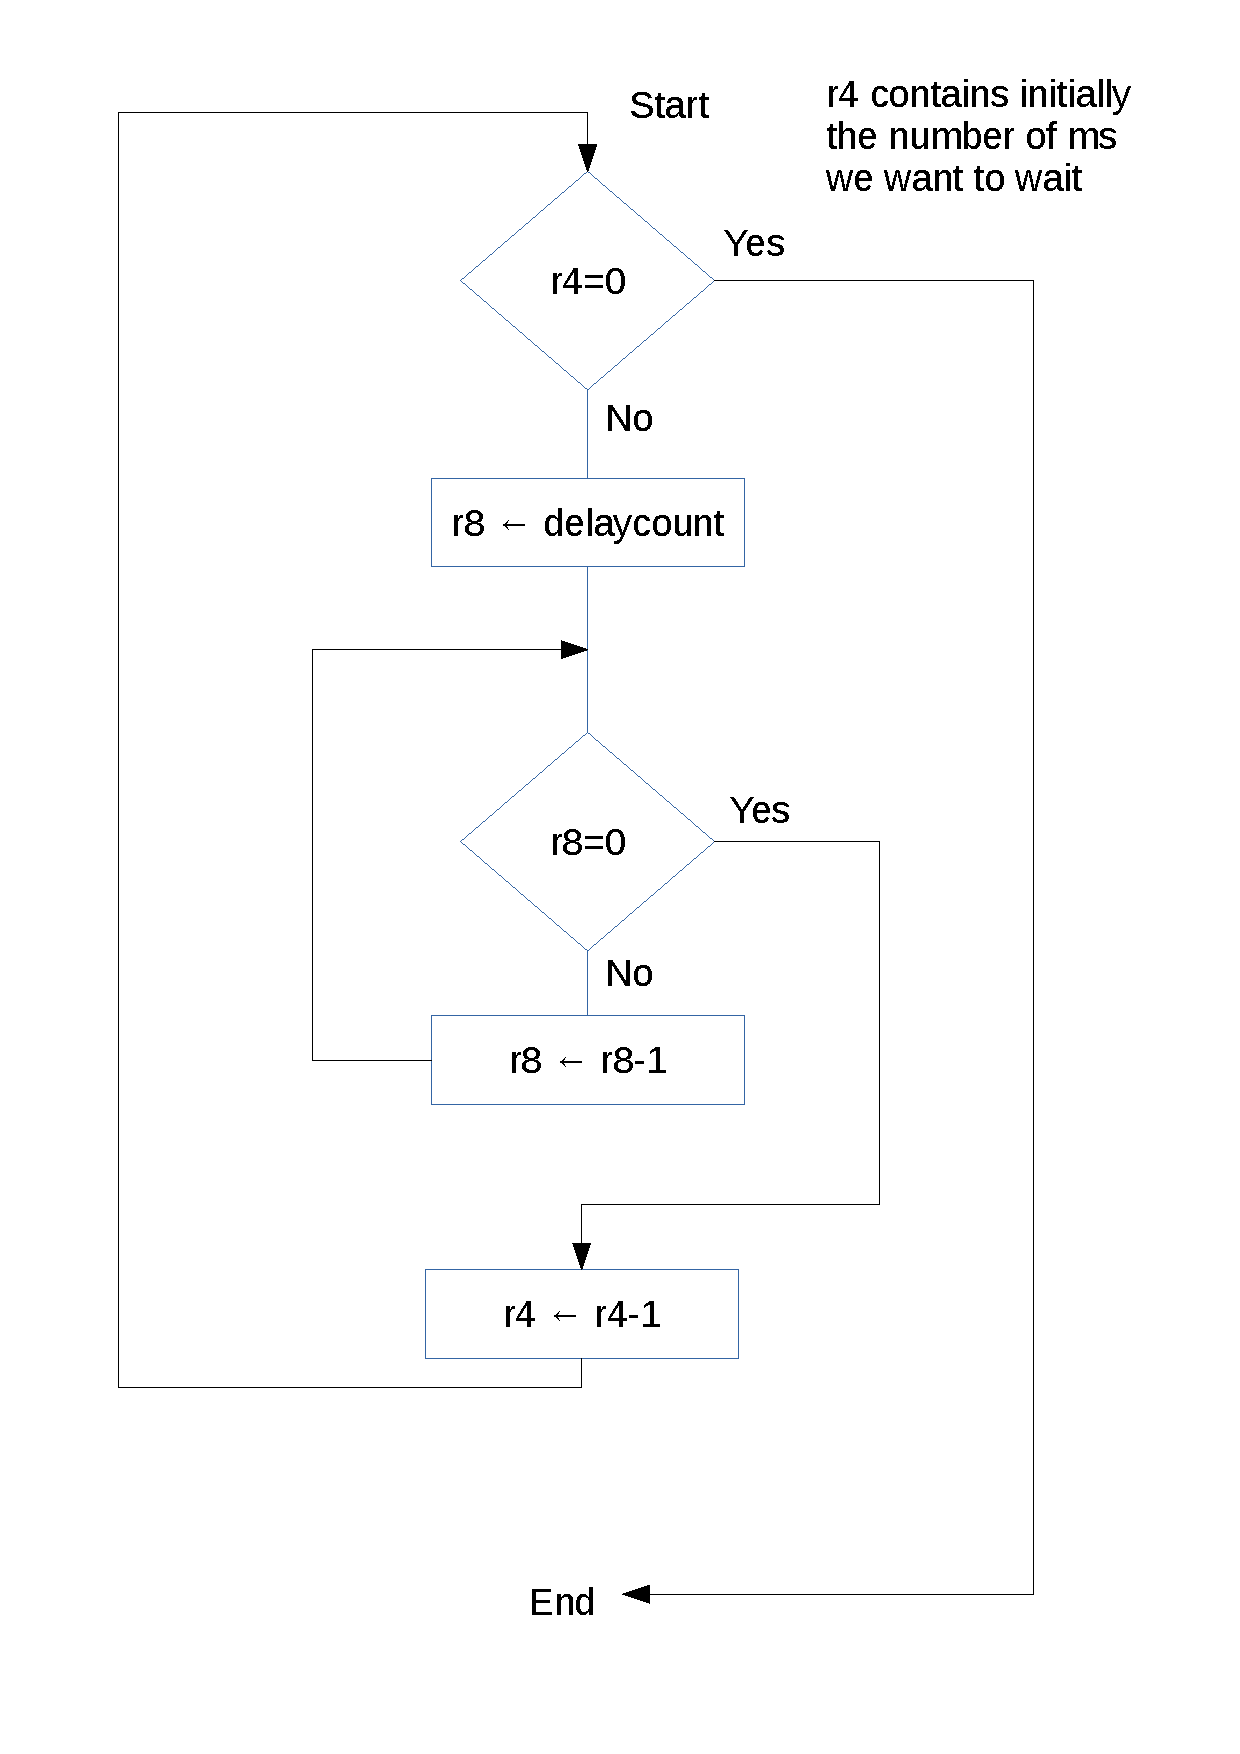
\includepdf[pages=-]{flow-diagram.pdf}


\end{document}
